% Options for packages loaded elsewhere
\PassOptionsToPackage{unicode}{hyperref}
\PassOptionsToPackage{hyphens}{url}
\PassOptionsToPackage{dvipsnames,svgnames,x11names}{xcolor}
%
\documentclass[
]{agujournal2019}

\usepackage{amsmath,amssymb}
\usepackage{iftex}
\ifPDFTeX
  \usepackage[T1]{fontenc}
  \usepackage[utf8]{inputenc}
  \usepackage{textcomp} % provide euro and other symbols
\else % if luatex or xetex
  \usepackage{unicode-math}
  \defaultfontfeatures{Scale=MatchLowercase}
  \defaultfontfeatures[\rmfamily]{Ligatures=TeX,Scale=1}
\fi
\usepackage{lmodern}
\ifPDFTeX\else  
    % xetex/luatex font selection
\fi
% Use upquote if available, for straight quotes in verbatim environments
\IfFileExists{upquote.sty}{\usepackage{upquote}}{}
\IfFileExists{microtype.sty}{% use microtype if available
  \usepackage[]{microtype}
  \UseMicrotypeSet[protrusion]{basicmath} % disable protrusion for tt fonts
}{}
\makeatletter
\@ifundefined{KOMAClassName}{% if non-KOMA class
  \IfFileExists{parskip.sty}{%
    \usepackage{parskip}
  }{% else
    \setlength{\parindent}{0pt}
    \setlength{\parskip}{6pt plus 2pt minus 1pt}}
}{% if KOMA class
  \KOMAoptions{parskip=half}}
\makeatother
\usepackage{xcolor}
\setlength{\emergencystretch}{3em} % prevent overfull lines
\setcounter{secnumdepth}{5}
% Make \paragraph and \subparagraph free-standing
\makeatletter
\ifx\paragraph\undefined\else
  \let\oldparagraph\paragraph
  \renewcommand{\paragraph}{
    \@ifstar
      \xxxParagraphStar
      \xxxParagraphNoStar
  }
  \newcommand{\xxxParagraphStar}[1]{\oldparagraph*{#1}\mbox{}}
  \newcommand{\xxxParagraphNoStar}[1]{\oldparagraph{#1}\mbox{}}
\fi
\ifx\subparagraph\undefined\else
  \let\oldsubparagraph\subparagraph
  \renewcommand{\subparagraph}{
    \@ifstar
      \xxxSubParagraphStar
      \xxxSubParagraphNoStar
  }
  \newcommand{\xxxSubParagraphStar}[1]{\oldsubparagraph*{#1}\mbox{}}
  \newcommand{\xxxSubParagraphNoStar}[1]{\oldsubparagraph{#1}\mbox{}}
\fi
\makeatother


\providecommand{\tightlist}{%
  \setlength{\itemsep}{0pt}\setlength{\parskip}{0pt}}\usepackage{longtable,booktabs,array}
\usepackage{calc} % for calculating minipage widths
% Correct order of tables after \paragraph or \subparagraph
\usepackage{etoolbox}
\makeatletter
\patchcmd\longtable{\par}{\if@noskipsec\mbox{}\fi\par}{}{}
\makeatother
% Allow footnotes in longtable head/foot
\IfFileExists{footnotehyper.sty}{\usepackage{footnotehyper}}{\usepackage{footnote}}
\makesavenoteenv{longtable}
\usepackage{graphicx}
\makeatletter
\def\maxwidth{\ifdim\Gin@nat@width>\linewidth\linewidth\else\Gin@nat@width\fi}
\def\maxheight{\ifdim\Gin@nat@height>\textheight\textheight\else\Gin@nat@height\fi}
\makeatother
% Scale images if necessary, so that they will not overflow the page
% margins by default, and it is still possible to overwrite the defaults
% using explicit options in \includegraphics[width, height, ...]{}
\setkeys{Gin}{width=\maxwidth,height=\maxheight,keepaspectratio}
% Set default figure placement to htbp
\makeatletter
\def\fps@figure{htbp}
\makeatother

\usepackage{url} %this package should fix any errors with URLs in refs.
\usepackage{lineno}
\usepackage[inline]{trackchanges} %for better track changes. finalnew option will compile document with changes incorporated.
\usepackage{soul}
\linenumbers
\makeatletter
\@ifpackageloaded{caption}{}{\usepackage{caption}}
\AtBeginDocument{%
\ifdefined\contentsname
  \renewcommand*\contentsname{Table of contents}
\else
  \newcommand\contentsname{Table of contents}
\fi
\ifdefined\listfigurename
  \renewcommand*\listfigurename{List of Figures}
\else
  \newcommand\listfigurename{List of Figures}
\fi
\ifdefined\listtablename
  \renewcommand*\listtablename{List of Tables}
\else
  \newcommand\listtablename{List of Tables}
\fi
\ifdefined\figurename
  \renewcommand*\figurename{Figure}
\else
  \newcommand\figurename{Figure}
\fi
\ifdefined\tablename
  \renewcommand*\tablename{Table}
\else
  \newcommand\tablename{Table}
\fi
}
\@ifpackageloaded{float}{}{\usepackage{float}}
\floatstyle{ruled}
\@ifundefined{c@chapter}{\newfloat{codelisting}{h}{lop}}{\newfloat{codelisting}{h}{lop}[chapter]}
\floatname{codelisting}{Listing}
\newcommand*\listoflistings{\listof{codelisting}{List of Listings}}
\makeatother
\makeatletter
\makeatother
\makeatletter
\@ifpackageloaded{caption}{}{\usepackage{caption}}
\@ifpackageloaded{subcaption}{}{\usepackage{subcaption}}
\makeatother

\ifLuaTeX
  \usepackage{selnolig}  % disable illegal ligatures
\fi
\usepackage{bookmark}

\IfFileExists{xurl.sty}{\usepackage{xurl}}{} % add URL line breaks if available
\urlstyle{same} % disable monospaced font for URLs
\hypersetup{
  pdftitle={Leading Ladies and Lost Revenue: A Causal Analysis of Female Representation and Box-Office Returns},
  pdfauthor={Lizzie Healy},
  pdfkeywords={Films, Gender Equality, Economics},
  colorlinks=true,
  linkcolor={blue},
  filecolor={Maroon},
  citecolor={Blue},
  urlcolor={Blue},
  pdfcreator={LaTeX via pandoc}}


\journalname{Film Data Science}

\draftfalse

\begin{document}
\title{Leading Ladies and Lost Revenue: A Causal Analysis of Female
Representation and Box-Office Returns}

\authors{Lizzie Healy\affil{1}}
\affiliation{1}{Georgetown University, }
\correspondingauthor{Lizzie Healy}{emh201@georgetown.com}


\begin{abstract}
This work will investigate the impact of gender bias in the film
industry pertaining to economic outcomes. Specifically, it will
establish a causal link between a film casting a female actress in the
leading role and the resulting box-office revenue. This will be
accomplished utilizing propensity weighting, which will match movies
based on the perceived similarity of their characteristics. These
predictor variables will include the year, season of release, genre,
runtime, director and writers, star power level of the cast, MPAA
rating, IMDb Metascore, IMDb Votes, number of awards won, country of
release, language, film description, the production budget, the aspect
ratio, the color, the countries of origin, filming locations, production
companies, and tagline. To deal with the variables that are non-numeric
the following steps will be taken. Firstly, a manufactured metric will
be created to capture the preceived `starpower' of the actors/actresses.
Secondly, a sentiment analysis will be performed on the film description
and tagline. The primary outcome variable will be the box-office number
measured in US dollars, measured as the gross value worldwide. The IMDb
score will be employed as an additional outcome measure to be used as a
robustness check. A secondary robustness check may be employed in which
the primary variable of interest will be whether the film passes the
Bechdel test, indicating true female representation in the film. The
initial hypothesis is that films that opt to feature a female in the
leading role will experience a decrease value in the box office revenue.
\end{abstract}

\section*{Plain Language Summary}
Propensity scoring regression analysis to determine whether female
versus male leads have a causal impact on the box office revenue and
IMDb rating of a film.




\section{Introduction}\label{introduction}

\textsubscript{Source:
\href{https://ehealy19.github.io/Matching_Movies/index.qmd.html}{Article
Notebook}}

\subsection{Causality}\label{causality}

My previous paper: \href{./assets/thesis.pdf}{Behind the Box Office:
Directorial Influence on Film Revenue in the United States Entertainment
Industry} attempted to analyze the link between director quality and
box-office success of a film. The paper created two novel measures of
director quality; a summation of all box-office revenue earned by and
the director's films and the accumulated number of critical awards from
the fifteen years leading up to the film in question. The main dependent
variable was domestic box-office revenue and a robustness check was
implemented changing the dependent variable to the IMDb rating earned.

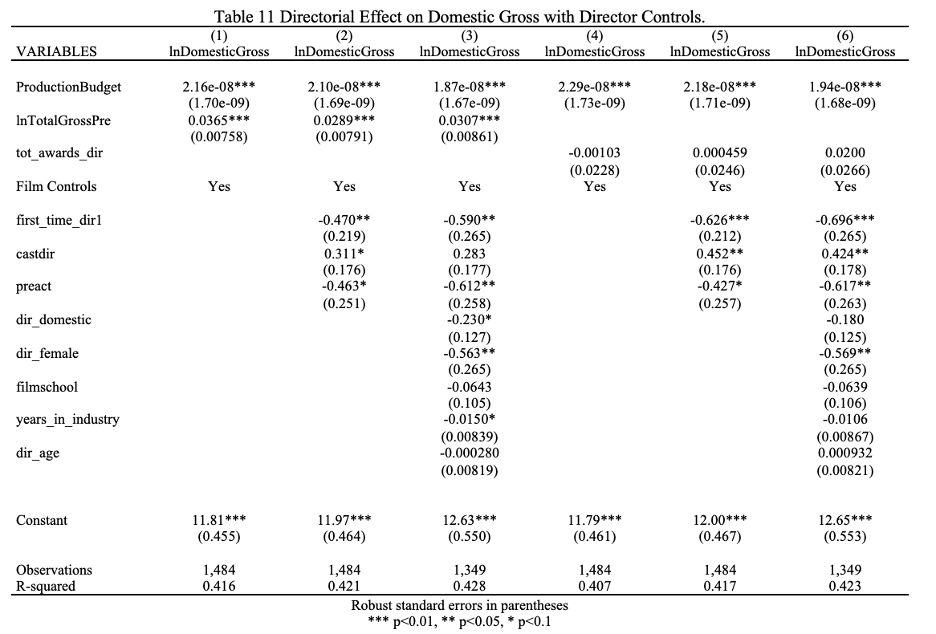
\includegraphics{./assets/thesis_table1.png}
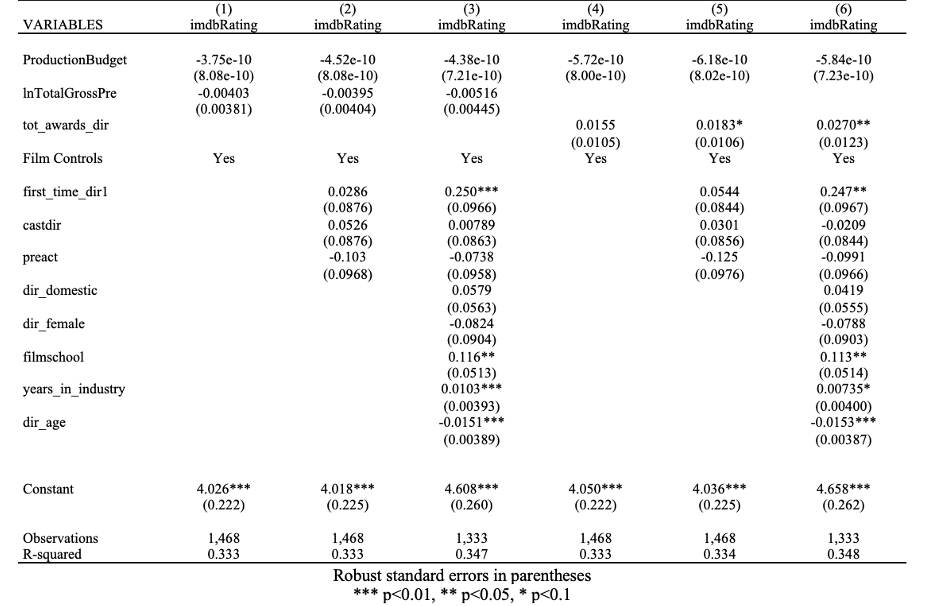
\includegraphics{./assets/thesis_table2.png}

The paper found an increase in director financial quality yielded
between a 0.0289\% and 0.0307\% increas in domestic gross and no impact
on IMDb rating. Conversely, director quality in terms of critical
acclaim yielded no significant impact on domestic gross, but betweeen
0.01803 and 0.0270 point increase in IMDb rating. The paper also
discovered a statistically significant decrease in domestic gross for
demale directors as compared to male directors.

Overall, the results were thought-provoking, however, the methodology
used was lacking in the causality department. This paper, if anything,
worked towards establishing a weak association due to it statical
analysis going only so far as a simple ordinary-least-squares regression
and controlling for confounding variables. While, the variables were
considered and included in the regression equation, they were all
treated equally as controls, thus a more complex analysis is warranted.

Furthermore, I wanted to investigate the conclusion of gender bias
further and shifted this analysis to examine actors instead of
directors.

Moving forward, the work to get to causality includes introducing
causality instead of just controlling for all covariates.

Thus, this paper will investigate the impact of gender bias in the film
industry pertaining to economic outcomes. Specifically, it will attempt
to establish a causal link between a film casting a female actress in
the leading role and the resulting box-office revenue by employing
propensity score matching.

Need to argue that there is sufficient common support between the
treatment and control groups in a dataset in order to use propensity
scores.

Data collection and preparation is discussed in Section~\ref{sec-data}.

Methodology and propensity scoring is discussed in
Section~\ref{sec-meth}

Results and anlysis are disucssed in Section~\ref{sec-results}

Conluding remarks, limitations, and future work are discussed in
Section~\ref{sec-conclusion}

\section{Data}\label{sec-data}

The data for this research was collected from separate sources:
\href{https://www.omdbapi.com/}{Open Movie Database (OMDb)} and
\href{https://www.themoviedb.org/}{The Movie Database (TMDb)}. Both are
sources for movie and television metadata, differing only in their
sourcing and specific variables provided. OMDb partly sources from
Amazon's Internet Movie Database (IMDb) and then relies on crowdsourcing
for missing data, while TMDb is independently created and relies solely
on crowd-sourcing from its community of film-buffs to provide data entry
for films. Both of these sources offer an API that allowed for the
collection of movie metadata, which was then merged using an inner join
on the film Title and resulted in the following variables: Title, Year,
Runtime, Budget, Released, Genre (Action, Adventure, Animation,
Biography, Comedy, Crime, Documentary, Drama, Family, Fantasy, Film
Noir, History, Horror, Music, Musical, Mystery, Romance, Sci-Fi, Sport,
Thriller, War, Western), MPAA Rating (G, GP, M, M/PG, NC-17, Not-Rated,
PG, PG-13, R, TV-MA, Unrated, Accepted), Production Companies, Director,
Writer, Country, Language, Description, Tagline, Overview, Actors, Box
Office, Revenue, IMDb Rating, Metascore, IMDb Votes, TMDb rating, Vote
Count, Awards, and Poster URL.

With this combined dataset, some further preparation was required to
move forward with the analysis. Firstly, some variables were dropped as
they were deemed unimportant while others were very similar across the
datasets for example only the description variable was kept and the
overview variable was dropped. All missing and zero values in numerical
variables were removed and each of the variables was converted to the
correct data type. The release date was split into three variables for
the month, day, and year. For the categorical variables two different
techniques were utilized. For the genere and MPAA rating a one-hot
encoding was applied. However for the language and country variables,
only the first observation of each was kept and then they were
categorized simply as either english or other language and domestic (for
US) and international for all other countries.

The final dataset included a total of 2,816 films with 61 columns of
variables.

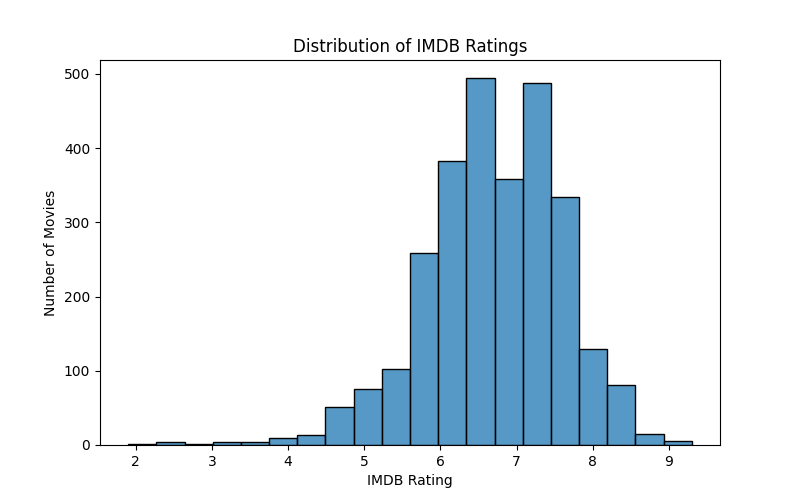
\includegraphics{./notebooks/notebook_output/imdb_rating.png}

\begin{longtable}[]{@{}lll@{}}
\caption{IMDb Rating Distribution}\label{tbl-1}\tabularnewline
\toprule\noalign{}
Variable & Minimum & Maximum \\
\midrule\noalign{}
\endfirsthead
\toprule\noalign{}
Variable & Minimum & Maximum \\
\midrule\noalign{}
\endhead
\bottomrule\noalign{}
\endlastfoot
Box Office & 3,622 & 858,373,000 \\
Budget & 7,000 & 460,000,000 \\
Runtime & 63 & 238 \\
IMDb Rating & 1.9 & 9.3 \\
IMDb Votes & 1,672 & 3,059,994 \\
\end{longtable}

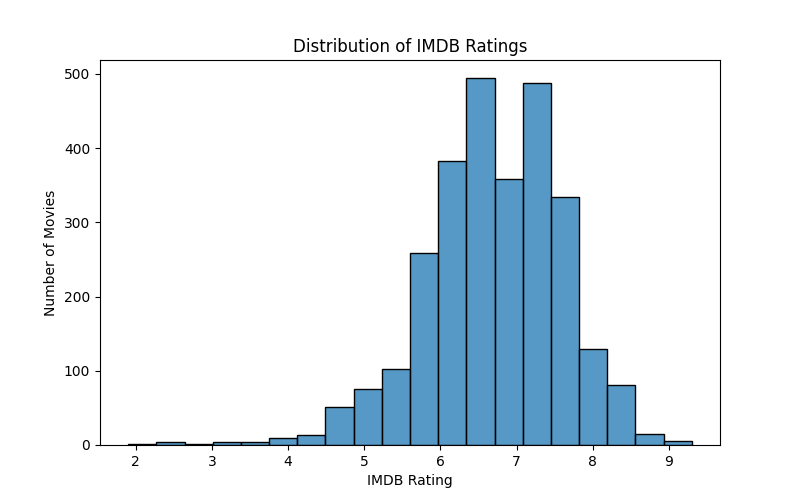
\includegraphics{./notebooks/notebook_output/imdb_rating.png}

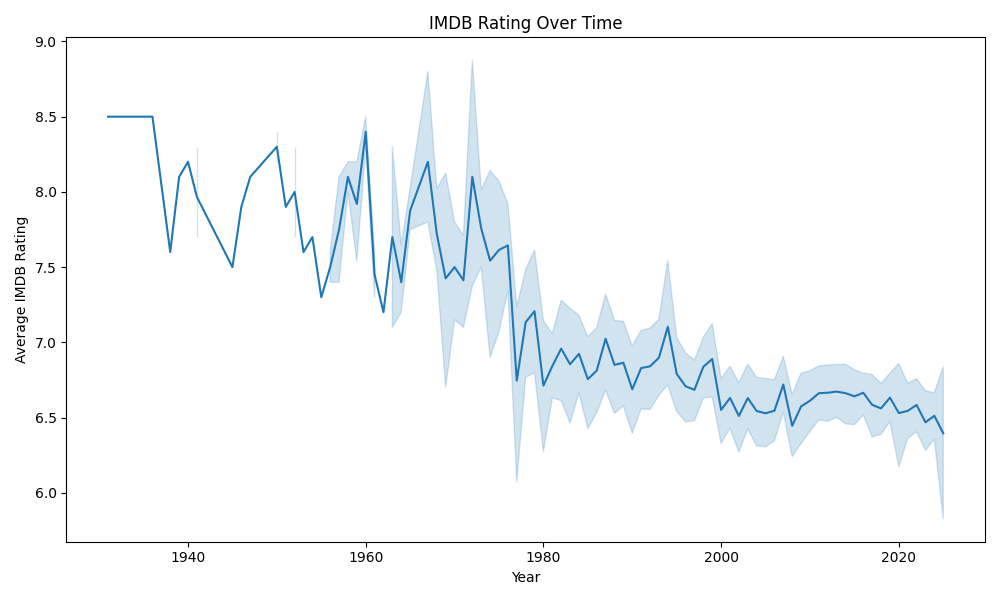
\includegraphics{./notebooks/notebook_output/imdb_overtime.png}
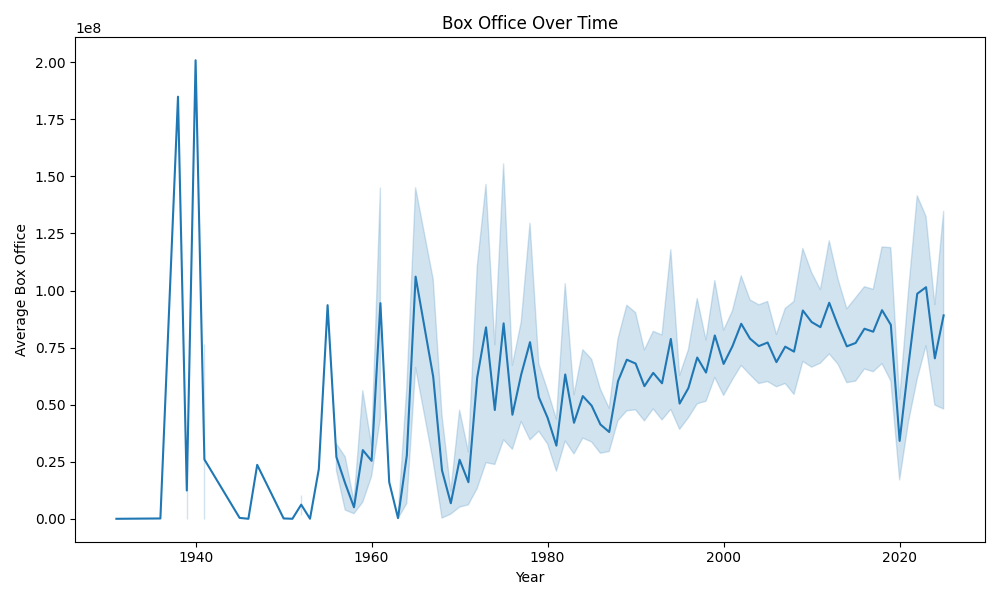
\includegraphics{./notebooks/notebook_output/boxoffice_overtime.png}

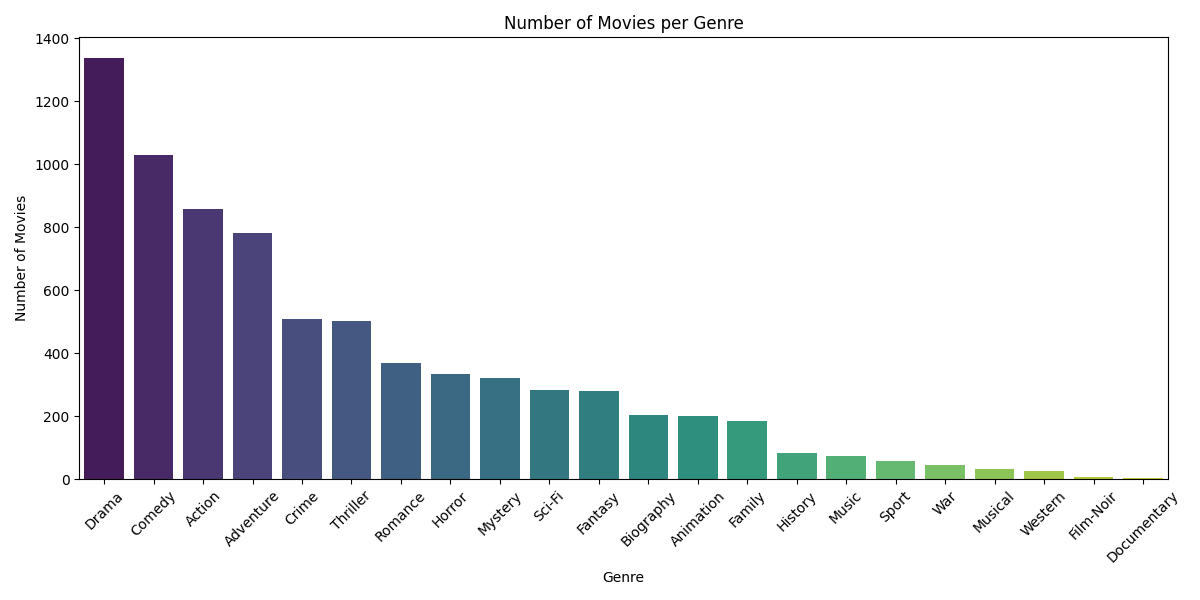
\includegraphics{./notebooks/notebook_output/genre_counts.png}
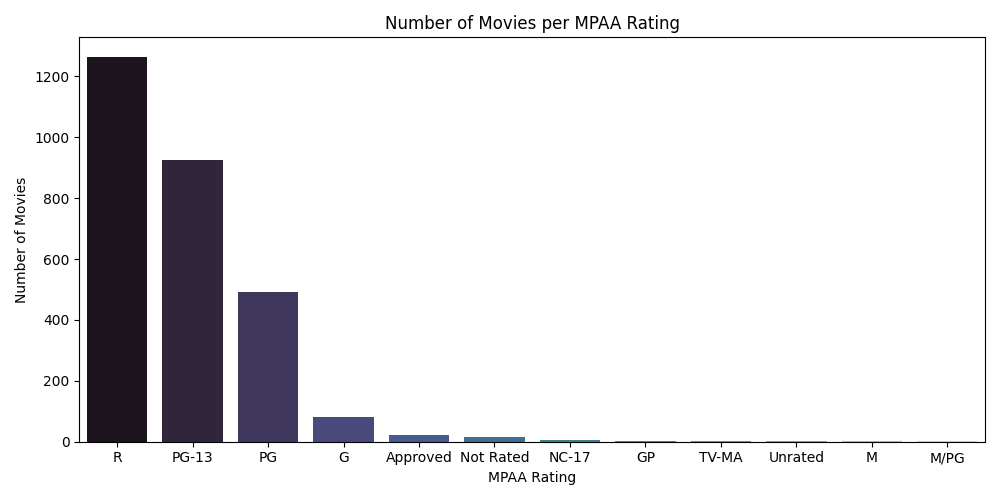
\includegraphics{./notebooks/notebook_output/rated_counts.png}

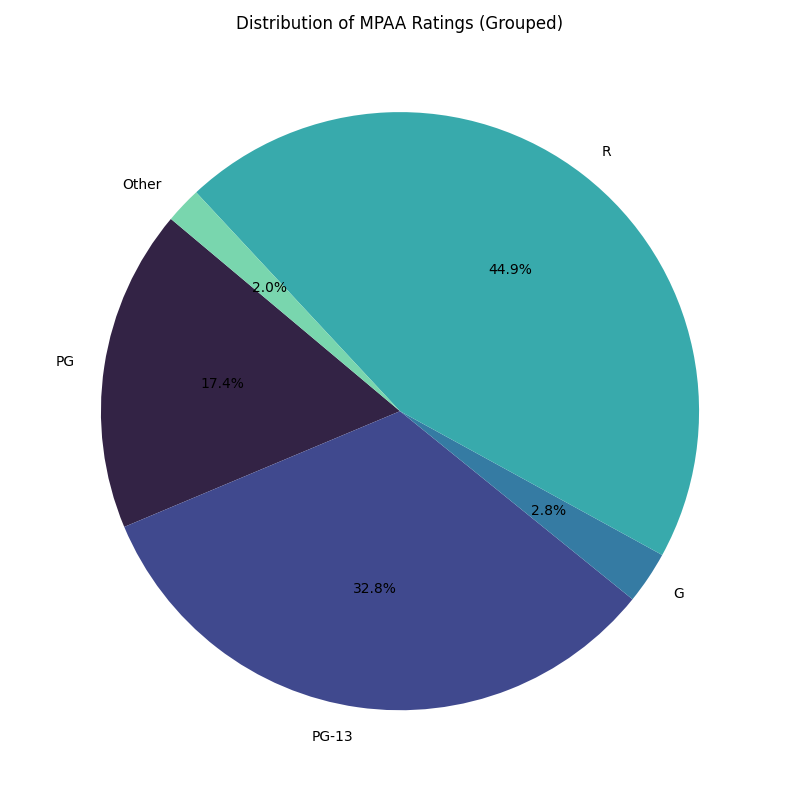
\includegraphics{./notebooks/notebook_output/mpaa_pie.png}

\section{Methodology}\label{sec-meth}

\subsection{Manufactured Variables}\label{manufactured-variables}

\subsubsection{Top Directors, Writers, Production
Companies}\label{top-directors-writers-production-companies}

In order to incorporate the level of expertise of the team creating the
film, this analysis worked to categorize top level of directors,
writers, and production companies. All of these were attempting to
better match movies based on the level of effort put into the creation
in terms of money, knowledge, experience, and previous success. To
achieve this, three lists were collected that detailed the top
directors, writers, and production companies:

\href{https://www.imdb.com/list/ls052380992/}{IMDb list of top
directors}\\
\href{https://www.imdb.com/list/ls064457317/}{IMDb list of top Script
writers}\\
\href{https://www.the-numbers.com/movies/production-companies/\#production_companies_overview=od1}{The
Numbers Top Production Companies}

The directors and writers were judged on a combination of their
perceived skill and their lifetime achievement in terms of awards and
accolades. The production companies were compiled simply based on the
total domestic box office revenue amassed across all films they have
produced.

The director, writer, and production company variable was then
referenced against these lists receiving a 1 if the entity was mentioned
in the list and a 0 otherwise, resulting in three one-hot encoded
variables: \texttt{Top\_Production}, \texttt{Top\_Director}, and
\texttt{Top\_Writer}. For the sake of simplicity if more than one entity
was listed for any of these variables, only the first entity was taken
into account.

\subsubsection{Sentiment Analysis of tagline and
description}\label{sentiment-analysis-of-tagline-and-description}

In order to extract meaningful value from the film description and
tagline, sentiment analysis was performed on the text. This sentiment
analyis was performed by an off-the-shelf pre-trained model publically
available
\href{https://huggingface.co/distilbert/distilbert-base-uncased-finetuned-sst-2-english}{Hugging
Face}. This model was trained on English text specifically for binary
text classifaction and boosted a high accuracy score. The end result is
a two variables with a binary value of 1 for positive sentiment or 0 for
negative sentiment of both the film description and film tagline.

\begin{longtable}[]{@{}
  >{\raggedright\arraybackslash}p{(\columnwidth - 6\tabcolsep) * \real{0.3014}}
  >{\raggedright\arraybackslash}p{(\columnwidth - 6\tabcolsep) * \real{0.2877}}
  >{\raggedright\arraybackslash}p{(\columnwidth - 6\tabcolsep) * \real{0.2466}}
  >{\raggedright\arraybackslash}p{(\columnwidth - 6\tabcolsep) * \real{0.1644}}@{}}
\caption{Example of the Tagline Sentiment
Values.}\label{tbl-1}\tabularnewline
\toprule\noalign{}
\begin{minipage}[b]{\linewidth}\raggedright
Title
\end{minipage} & \begin{minipage}[b]{\linewidth}\raggedright
Tagline
\end{minipage} & \begin{minipage}[b]{\linewidth}\raggedright
Tagline Sentiment
\end{minipage} & \begin{minipage}[b]{\linewidth}\raggedright
\end{minipage} \\
\midrule\noalign{}
\endfirsthead
\toprule\noalign{}
\begin{minipage}[b]{\linewidth}\raggedright
Title
\end{minipage} & \begin{minipage}[b]{\linewidth}\raggedright
Tagline
\end{minipage} & \begin{minipage}[b]{\linewidth}\raggedright
Tagline Sentiment
\end{minipage} & \begin{minipage}[b]{\linewidth}\raggedright
\end{minipage} \\
\midrule\noalign{}
\endhead
\bottomrule\noalign{}
\endlastfoot
Surf's Up & A Major Ocean Picture. & 1 & \\
The BFG & The world is more giant than you can imagine. & 1 & \\
Twin Peaks: Fire Walk with Me & In a town like Twin Peaks, no one is
innocent. & 0 & \\
Meet the Robinsons & If you think your family's different, wait 'til you
meet the family of the future. & 1 & \\
The Royal Tenenbaums & Family isn't a word \ldots{} It's a sentence. & 0
& \\
\end{longtable}

\begin{longtable}[]{@{}ll@{}}
\caption{Count of positive and negative
sentiment.}\label{tbl-1}\tabularnewline
\toprule\noalign{}
Sentiment & Count \\
\midrule\noalign{}
\endfirsthead
\toprule\noalign{}
Sentiment & Count \\
\midrule\noalign{}
\endhead
\bottomrule\noalign{}
\endlastfoot
Positive & 1476 \\
Negative & 1340 \\
\end{longtable}

\subsubsection{Creation of the starpower
variable}\label{creation-of-the-starpower-variable}

One of the most important building blocks of a film is the cast of
actors and actresses and well-known names can be a huge draw to the
theatres to movie-goers. This feature seemingly has an impact on the
outcome of the film and its financial success. Thus, finding a way to
classify the `starpowerness' of the cast was paramount to this analysis.
The dataset, unfortunately, only provides the three main cast members,
which discounts films that rely on an ensemble cast or have a large
enough budget to cast many big-names. That being said, this research
attempted to define a metric that quantified this `starpower' aspects of
the three cast members, in the hopes that the success and
name-recognition can be at least partly captured.

The metric was created by the collecting lists of A-list and B-list
actors and actresses. In film-terms these categorization reflect how
`bankable' the stars are or how many financial draw they bring to a film
theoretically. These lists are all collected from IMDb and included a
wide-range of household names. With these lists, the cast variable was
split into actor1, actor2, actor3 based simply on the order in which
they were listed. Then, each of the cast variables were referenced
against all three of the lists. The film title received:

\begin{itemize}
\tightlist
\item
  \textbf{2 points} if a cast member was part of the A-list\\
\item
  \textbf{1 point} if cast member was part of the B-list
\end{itemize}

These points were added in the \texttt{starpower} variable and then
divided by three to get a finalized score of the points across the three
cast members. Table~\ref{tbl-5} shows an example of the scoring.

\begin{longtable}[]{@{}
  >{\raggedright\arraybackslash}p{(\columnwidth - 6\tabcolsep) * \real{0.3014}}
  >{\raggedright\arraybackslash}p{(\columnwidth - 6\tabcolsep) * \real{0.2877}}
  >{\raggedright\arraybackslash}p{(\columnwidth - 6\tabcolsep) * \real{0.2466}}
  >{\raggedright\arraybackslash}p{(\columnwidth - 6\tabcolsep) * \real{0.1644}}@{}}
\caption{Starpower metric scores for actors in 10
movies.}\label{tbl-5}\tabularnewline
\toprule\noalign{}
\begin{minipage}[b]{\linewidth}\raggedright
actor1
\end{minipage} & \begin{minipage}[b]{\linewidth}\raggedright
actor2
\end{minipage} & \begin{minipage}[b]{\linewidth}\raggedright
actor3
\end{minipage} & \begin{minipage}[b]{\linewidth}\raggedright
starpower
\end{minipage} \\
\midrule\noalign{}
\endfirsthead
\toprule\noalign{}
\begin{minipage}[b]{\linewidth}\raggedright
actor1
\end{minipage} & \begin{minipage}[b]{\linewidth}\raggedright
actor2
\end{minipage} & \begin{minipage}[b]{\linewidth}\raggedright
actor3
\end{minipage} & \begin{minipage}[b]{\linewidth}\raggedright
starpower
\end{minipage} \\
\midrule\noalign{}
\endhead
\bottomrule\noalign{}
\endlastfoot
Mark Wahlberg & Tyrese Gibson & André 3000 & 0.666667 \\
Jamie Bell & Andy Serkis & Daniel Craig & 1.333333 \\
Ryan Reynolds & Blake Lively & Peter Sarsgaard & 0.333333 \\
Marc Singer & Tanya Roberts & Rip Torn & 0.000000 \\
Tom Hiddleston & Samuel L. Jackson & Brie Larson & 1.000000 \\
Jeremy Renner & Ed Helms & Jake Johnson & 0.000000 \\
Frankie Muniz & Amanda Bynes & Paul Giamatti & 1.000000 \\
Ben Barnes & Skandar Keynes & Georgie Henley & 0.000000 \\
Jason Bateman & Charlie Day & Jason Sudeikis & 1.000000 \\
Jack Black & Ana de la Reguera & Héctor Jiménez & 0.333333 \\
\end{longtable}

\href{https://www.imdb.com/list/ls056262001/}{IMDb A-list Actors}
\href{https://www.imdb.com/list/ls056262192/}{IMDb A-list Actresses}
\href{https://www.imdb.com/list/ls024783564/}{IMDb B-list}

\subsubsection{Creation of the variable that indicates female in leading
role}\label{creation-of-the-variable-that-indicates-female-in-leading-role}

This analysis relied on the ability to distinguish between female and
male leading actresses and actors, however, this is not something
directly encoded into the metadata of a film, thus this variable had to
be manufactured. In order to achieve this, a list of all current female
actresses was collected from
\href{https://en.wikipedia.org/wiki/List_of_American_film_actresses}{Wikipedia}.
This list included 2,816 names of female actresses, alphabetized. To
note, there was attempts to utilize a list of all female names and an
off-the-shelf model to guess whether the cast member listed identified a
male of female, however, both of these methods produced increased
inaccuracy, thus the list of female actresses method was proceeded with.

The next step was to determine only the presumed lead cast member by
extracting the first person listed in the `Actors' variable of the
dataset. This name was then compared against the list from of female
actresses and received a value of 1 if the cast member was included on
the list.

Therefore, the end result was a variable titled `female\_lead' if the
first cast member listed in the IMDb metadata was a member of the
current working female actress list and a 0 if the cast member was not a
member of the list and, thus, presumably a male actor. Table~\ref{tbl-1}
displays an example of the accuracy results of this variable.

\begin{longtable}[]{@{}lll@{}}
\caption{Example of the `female\_lead'
variable}\label{tbl-1}\tabularnewline
\toprule\noalign{}
Title & First Actor & Female Lead \\
\midrule\noalign{}
\endfirsthead
\toprule\noalign{}
Title & First Actor & Female Lead \\
\midrule\noalign{}
\endhead
\bottomrule\noalign{}
\endlastfoot
The Family & Robert De Niro & 0 \\
The Shack & Sam Worthington & 0 \\
The Dead Zone & Christopher Walken & 0 \\
The Ref & Denis Leary & 0 \\
Flyboys & James Franco & 0 \\
ATL & Tip `T.I.' Harris & 0 \\
Like a Boss & Tiffany Haddish & 1 \\
Enemy Mine & Dennis Quaid & 0 \\
Proud Mary & Taraji P. Henson & 1 \\
Valmont & Colin Firth & 0 \\
\end{longtable}

As displayed in Table~\ref{tbl-2} the films were split between 488 films
with female leading actresses and 2328 films with male leading actors.

\begin{longtable}[]{@{}ll@{}}
\caption{Male versus Female Director}\label{tbl-2}\tabularnewline
\toprule\noalign{}
Name & Year \\
\midrule\noalign{}
\endfirsthead
\toprule\noalign{}
Name & Year \\
\midrule\noalign{}
\endhead
\bottomrule\noalign{}
\endlastfoot
Female Leads & 488 \\
Male Leads & 2328 \\
\end{longtable}

\subsection{Propensity score matching}\label{propensity-score-matching}

The primary statistical analysis performed was propensity score matching
(PSM). This statistical method allows for comparison of films that are
similar across all observed covariates, differing only in whether the
lead is a male or female actor or actress. In this context, the presence
of a female lead is handled as a treatment, and the effect of that
treatement on the outcome variable is estimated.

Unlike simply including covariates as controls in a regression equation,
this technique aims to reduce selection bias by matching treated and
control units based on their likelihood of receiving the treatment,
given the covariates. This creates a more comparable dataset, which
quasi-miimcks the conditions of a randomized experiment.

The process of propensity score matching began with normalizing the
variables due to the very differing range of values across variables
like the imdb rating (which is 0-10) and the budget (which can reach
hundreds of millions). This was done with
\href{https://scikit-learn.org/stable/modules/generated/sklearn.preprocessing.StandardScaler.html}{Sklearn's
StandardScaler} and performed on all numerical variables.

Following this step, the variance inflation factor (VIF) was checked to
investigate any multicollinearity issues amoung that the covariates that
would bias the analysis. This yields some problematic variables, which
resulted in excluding some variables that exceeded the VIF threshold of
10 points. The following variables were excluded: international country
(domestic country kept), other language (English kept), musical genre
(all other genre categories kept), and accepted MPAA rating (all other
MPAA ratings kept).

Next, a logistic regression is estimated. The variables metascore, IMDb
votes, TMDb rating, TMDb votes, Oscars Won, Oscars Nominated, Award
Wins, and Award Nominations are omitted because they are ex-post
variables because they represent effects of the outcomes as oppose to
causes of it, thus causing data leakage and bias. Therefore, only
ex-ante variables are considered. The resulting equation is as follows,
representing a female leading role as the treatment and the film
characteristics as covariates:

\begin{align}
\text{logit}(\mathbb{P}(\text{Female\_Lead} = 1)) &= \beta_0 
+ \beta_1 \cdot \text{Year}
+ \beta_2 \cdot \text{Runtime}
+ \beta_3 \cdot \text{Budget}
+ \beta_4 \cdot \text{Month}
+ \beta_5 \cdot \text{Day} \nonumber \\
&\quad + \sum_{g} \beta_g \cdot \text{Genre}_g
+ \sum_{r} \beta_r \cdot \text{Rating}_r \nonumber \\
&\quad + \beta_6 \cdot \text{Top\_Production\_Company}
+ \beta_7 \cdot \text{Top\_Director}
+ \beta_8 \cdot \text{Top\_Writer} \nonumber \\
&\quad + \beta_9 \cdot \text{Domestic}
+ \beta_{10} \cdot \text{English\_Language} \nonumber \\
&\quad + \beta_{11} \cdot \text{Descr\_Sentiment}
+ \beta_{12} \cdot \text{Tagline\_Sentiment}
+ \beta_{13} \cdot \text{Starpower}
\end{align}

The result of this equation is propensity scores (ps) for each film
title (dataset row), which represents the calculated probability of the
film having a female leading actress. A score close to 0 indicates a
higher likelihood of the film having a male lead, while a score closer
to 1 indicates a higher likelihood of a film having a female lead. These
scores are then used to match, utilizing 1:1 nearest neighbor matching,
the movies across the two groups of leading actors/actresses based on
the closest propensity score. This results in a matched dataset with
each row being a matched pair of films that is similar in all aspects
expect for the leading role.

\begin{longtable}[]{@{}lll@{}}
\caption{Table}\label{tbl-2}\tabularnewline
\toprule\noalign{}
Female Led Movie & PS Female & Male Led Movie \\
\midrule\noalign{}
\endfirsthead
\toprule\noalign{}
Female Led Movie & PS Female & Male Led Movie \\
\midrule\noalign{}
\endhead
\bottomrule\noalign{}
\endlastfoot
Miss Congeniality & 0.082866 & Back to the Future Part III \\
GI Jane & 0.031775 & Gladiator \\
Freaky Friday & 0.212226 & The Boat the Rocked \\
Kill Bill: Vol. 2 & 0.066924 & 2 Fast 2 Furious \\
\end{longtable}

The final step is to calculate and compare the box office performance of
matched female versus male lead films. These results are discussed in
Section~\ref{sec-results}.

\subsection{Robustness Checks}\label{robustness-checks}

As a robustness check, the IMDb rating, which is a score from 0-10
calculated from a weighted average of user rating on the Internet Movie
Database, is utilized as a secondary outcome variable. The same
methodology of propensity score matching is used, however, the analysis
now investigates whether a female lead role causes a change in the
critical success of the film. These results are discussed in the
following section, Section~\ref{sec-results}.

\section{Results}\label{sec-results}

\begin{longtable}[]{@{}lll@{}}
\caption{Table}\label{tbl-2}\tabularnewline
\toprule\noalign{}
Gender of Lead Role & Box Office & IMDb Rating \\
\midrule\noalign{}
\endfirsthead
\toprule\noalign{}
Gender of Lead Role & Box Office & IMDb Rating \\
\midrule\noalign{}
\endhead
\bottomrule\noalign{}
\endlastfoot
Female & 62,708,871.36 & 6.329 \\
Male & 61,076,707.45 & 6.601 \\
\end{longtable}

\subsection{Box Office Results}\label{box-office-results}

Female-lead had higher box-office average

\subsection{IMDb Rating Results}\label{imdb-rating-results}

Female-lead had lower IMDb scores

\section{Conclusion}\label{sec-conclusion}

\subsection{Limitations:}\label{limitations}

\begin{enumerate}
\def\labelenumi{\arabic{enumi}.}
\tightlist
\item
  More data
\item
  Network Analysis
\item
  Robustness Checks with Bechdel test
\item
  Inacurracy from matching female leads \& first actor not always the
  lead
\item
  Unbalanced Dataset (is this an issue?) Further Work:
\item
  classify the tagline and description
\end{enumerate}

\section*{References}\label{references}
\addcontentsline{toc}{section}{References}

\vspace{1em}

\textsubscript{Source:
\href{https://ehealy19.github.io/Matching_Movies/index.qmd.html}{Article
Notebook}}




\end{document}
